\documentclass[11pt,a4paper]{article}
\usepackage[margin=2.1cm]{geometry}
\usepackage{amsmath,amssymb}
\usepackage{booktabs,tabularx,array}
\usepackage{xcolor}
\usepackage{tikz}
\usetikzlibrary{positioning,arrows.meta,calc}
\usepackage[hidelinks]{hyperref}
\usepackage{parskip}
\usepackage{enumitem}
\setlist{nosep,leftmargin=1.4em}

\definecolor{inp}{HTML}{2a78d6}
\definecolor{net}{HTML}{52514e}
\definecolor{form}{HTML}{eb6834}
\definecolor{phys}{HTML}{1baf7a}
\definecolor{loss}{HTML}{c0392b}
\definecolor{tgt}{HTML}{eda100}

\tikzset{
  box/.style={draw, rounded corners=2pt, align=center, font=\footnotesize, inner sep=4pt, minimum height=8mm, line width=0.7pt},
  inbox/.style={box, draw=inp, fill=inp!8},
  netbox/.style={box, draw=net, fill=net!8},
  formbox/.style={box, draw=form, fill=form!10},
  physbox/.style={box, draw=phys, fill=phys!10},
  lossbox/.style={box, draw=loss, fill=loss!8},
  tgtbox/.style={box, draw=tgt, fill=tgt!12},
  arr/.style={-{Latex[length=2mm]}, line width=0.7pt},
  darr/.style={-{Latex[length=2mm]}, line width=0.7pt, dashed},
}

\newcommand{\dz}{\Delta z}
\newcommand{\Shat}{\hat S}

\title{The network types in use}
\date{28 October 2026}
\author{}

\begin{document}
\begin{center}{\LARGE The network types in use}\end{center}
\vspace{2mm}

\begin{center}
\footnotesize
\begin{tabularx}{\textwidth}{@{}l X X l@{}}
\toprule
Type & The network emits & End of a step & Loss \\
\midrule
1 & the stage states & summed from the stages & pooled or cost-weighted \\
2 & the correction to the straight line, scaled per track & summed from the stages & pooled \\
3 & the correction to the straight line, one fixed scale & summed from the stages & pooled \\
\bottomrule
\end{tabularx}
\end{center}

Colours in the schematics:
\textcolor{inp}{\textbf{blue}} input,
\textcolor{net}{\textbf{grey}} network,
\textcolor{form}{\textbf{orange}} raw output to state,
\textcolor{phys}{\textbf{green}} physics with no trained weights,
\textcolor{loss}{\textbf{red}} loss,
\textcolor{tgt}{\textbf{yellow}} reference states.

\section{Common to all types}

\subsection*{State and equation of motion}

The region is $z_0 = 2648.2$\,mm to $z_1 = 7826.0$\,mm, length $L = 5177.8$\,mm. The state on a plane of constant $z$ is $S = (x, y, t_x, t_y, q/p)$. The rates are
\begin{align*}
\frac{dx}{dz} &= t_x, &
\frac{dt_x}{dz} &= \kappa\,\tfrac{q}{p}\,\sqrt{1+t_x^2+t_y^2}\,\bigl(t_x t_y B_x - (1+t_x^2) B_y + t_y B_z\bigr),\\
\frac{dy}{dz} &= t_y, &
\frac{dt_y}{dz} &= \kappa\,\tfrac{q}{p}\,\sqrt{1+t_x^2+t_y^2}\,\bigl((1+t_y^2) B_x - t_x t_y B_y - t_x B_z\bigr),
\end{align*}
with $d(q/p)/dz = 0$, $\kappa = 10^{-3}$, and $B$ from the field map. $q/p$ is an input to every step and is never predicted. Write $f(S, z)$ for the four rates.

\subsection*{One network, chained}

One network serves one step length $\dz = L/N$. It is applied $N$ times. Step $k$ starts on $z_k = z_0 + k\dz$. The end state of step $k$, with $q/p$ copied, is the input of step $k+1$. $\dz$ is a constant of the network, not an input.

\subsection*{The Gauss--Legendre step}

The network emits the $q$ stages of a Gauss--Legendre step (tableau $A$, weights $b$, nodes $c$). Stage $j$ is the state on the plane $z_k + c_j\dz$. The exact stages solve
\[
\Shat_j = S + \dz \sum_{m=1}^{q} A_{jm}\, f(\Shat_m,\ z_k + c_m \dz), \qquad j = 1,\dots,q.
\]
The end of the step is collected and summed from the stages:
\[
S_{\text{end}} = S + \dz \sum_{m=1}^{q} b_m\, f(\Shat_m,\ z_k + c_m \dz).
\]

\subsection*{The network body}

\begin{itemize}
\item 6 inputs: $S$ divided by the spread of each component over the round-1 training states, and $z_k$ mapped linearly onto $[-1, 1]$.
\item 2 hidden layers of 128 units, $\tanh$.
\item A linear output layer of $4q$ numbers: $q$ stages $\times$ $(x, y, t_x, t_y)$.
\item Double precision.
\end{itemize}

The types differ only in how the $4q$ raw outputs become stage states.

\subsection*{Tracks}

Simulated particles, each carried across the region by a sixth-order Runge--Kutta integrator at 0.1\,mm steps. The state is stored on 257 planes. This is the reference.

\begin{center}
\footnotesize
\begin{tabular}{@{}lrl@{}}
\toprule
Split & Tracks & Use \\
\midrule
training & 11,567 & round-1 states; start states of the chains in later rounds \\
validation & 1,463 & stopping rule \\
test & 1,452 & scores \\
\bottomrule
\end{tabular}
\end{center}

\subsection*{No labels}

The loss uses only the equation of motion and the network outputs. No reference state is in the loss. The reference is used for the round-1 training states, for validation, and for test.

\newpage
\section{How the data is fed}

Training is in rounds.

\begin{center}
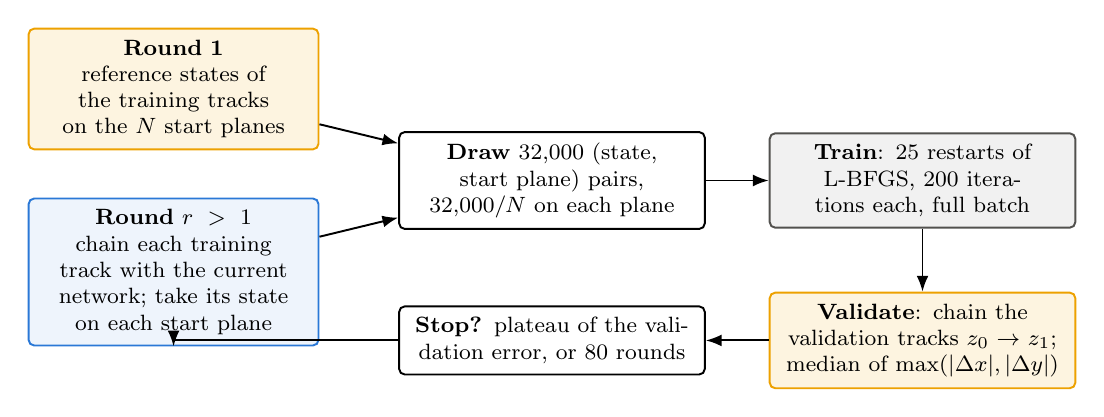
\begin{tikzpicture}[node distance=5mm and 6mm]
\node[tgtbox, text width=34mm] (r1) {\textbf{Round 1}\\reference states of the training tracks on the $N$ start planes};
\node[inbox, text width=34mm, below=6mm of r1] (rk) {\textbf{Round $r>1$}\\chain each training track with the current network; take its state on each start plane};
\coordinate (m) at ($(r1.east)!0.5!(rk.east)$);
\node[box, draw=black, text width=36mm, right=10mm of m] (draw) {\textbf{Draw} 32,000 (state, start plane) pairs, $32{,}000/N$ on each plane};
\node[netbox, text width=36mm, right=8mm of draw] (opt) {\textbf{Train}: 25 restarts of L-BFGS, 200 iterations each, full batch};
\node[tgtbox, text width=36mm, below=8mm of opt] (val) {\textbf{Validate}: chain the validation tracks $z_0 \to z_1$; median of $\max(|\Delta x|, |\Delta y|)$};
\node[box, draw=black, text width=36mm, left=8mm of val] (stop) {\textbf{Stop?} plateau of the validation error, or 80 rounds};
\draw[arr] (r1) -- (draw);
\draw[arr] (rk) -- (draw);
\draw[arr] (draw) -- (opt);
\draw[arr] (opt) -- (val);
\draw[arr] (val) -- (stop);
\draw[arr] (stop.west) -| (rk.south);
\end{tikzpicture}
\end{center}

\begin{itemize}
\item The 32,000 states of a round are fixed during the round.
\item Each state is one step on its own. No gradient flows through the chain.
\item From round 2 the network trains on the states its own chain visits.
\item The loss is rescaled to 1 at the start of each round, and again with a new optimiser each time it falls by a factor 10.
\item Plateau: the median validation error of the last 10 rounds is at least 0.95 of the median of the 10 before, at each of the last 3 rounds.
\item The input scales, the output scales of types 1 and 3, and the loss constants are measured once, on the round-1 states.
\end{itemize}

\newpage
\section{Type 1: direct stage states}

The network emits the stage states. A raw output of zero is the origin of the detector.

\begin{center}
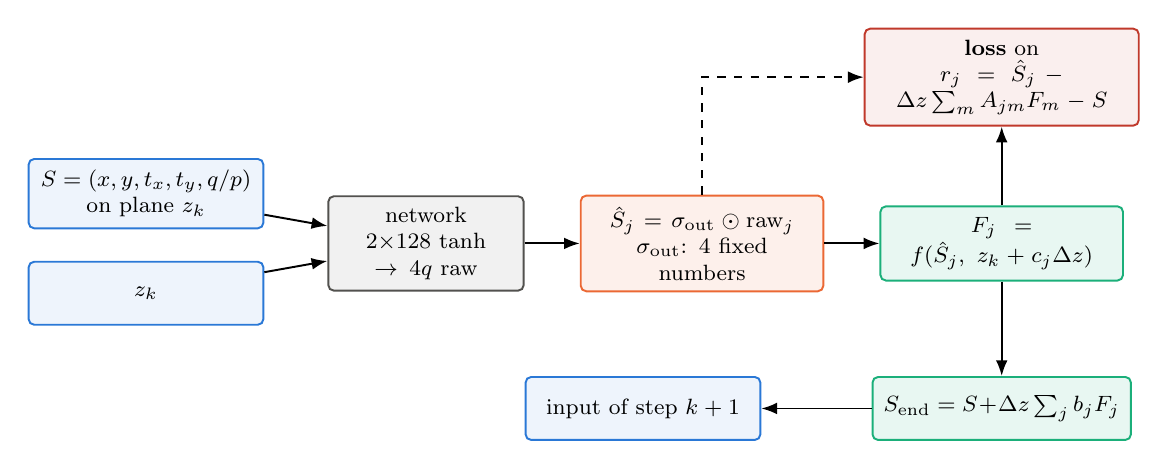
\begin{tikzpicture}[node distance=6mm and 7mm]
\node[inbox, text width=27mm] (S) {$S = (x, y, t_x, t_y, q/p)$\\on plane $z_k$};
\node[inbox, text width=27mm, below=4mm of S] (z) {$z_k$};
\coordinate (m) at ($(S.east)!0.5!(z.east)$);
\node[netbox, text width=22mm, right=8mm of m] (body) {network\\2$\times$128 tanh\\$\to 4q$ raw};
\node[formbox, text width=28mm, right=of body] (form) {$\Shat_j = \sigma_{\text{out}} \odot \text{raw}_j$\\$\sigma_{\text{out}}$: 4 fixed numbers};
\node[physbox, text width=28mm, right=of form] (rates) {$F_j = f(\Shat_j,\ z_k + c_j\dz)$};
\node[physbox, text width=30mm, below=12mm of rates] (sum) {$S_{\text{end}} = S + \dz\sum_j b_j F_j$};
\node[inbox, text width=27mm, left=14mm of sum] (next) {input of step $k+1$};
\node[lossbox, text width=32mm, above=10mm of rates] (loss) {\textbf{loss} on\\$r_j = \Shat_j - \dz\sum_m A_{jm}F_m - S$};
\draw[arr] (S) -- (body); \draw[arr] (z) -- (body);
\draw[arr] (body) -- (form);
\draw[arr] (form) -- (rates);
\draw[arr] (rates) -- (sum);
\draw[arr] (sum) -- (next);
\draw[arr] (rates) -- (loss);
\draw[darr] (form.north) |- (loss.west);
\end{tikzpicture}
\end{center}

\begin{center}
\footnotesize
\begin{tabularx}{\textwidth}{@{}l X@{}}
\toprule
Input & $S$ and $z_k$. \\
Raw output & $4q$ numbers. \\
Prediction & The $q$ stage states: $\Shat_j = \sigma_{\text{out}} \odot \text{raw}_j$. $\sigma_{\text{out}}$ is the spread of $(x, y, t_x, t_y)$ over the round-1 states (445\,mm, 365\,mm, 0.164, 0.069 at $N = 64$). \\
End of step & $S + \dz\sum_j b_j f(\Shat_j, z_k + c_j\dz)$. \\
Target & None. \\
Loss & Pooled or cost-weighted, on the $q$ stage residuals. \\
Configurations & 64 steps / 2 stages, 128 / 8, 256 / 16. \\
\bottomrule
\end{tabularx}
\end{center}

\newpage
\section{Type 2: straight line plus a correction, scaled per track}

The network emits the correction to the straight line. The correction is multiplied by a scale computed for each track from its state and the field along its straight line. A raw output of zero is the straight line.

\begin{center}
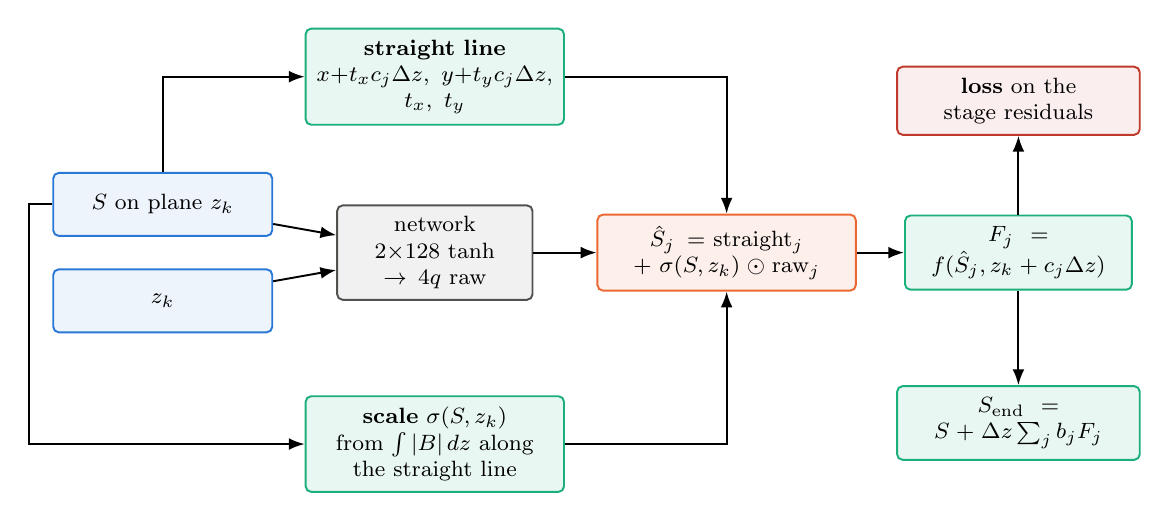
\begin{tikzpicture}[node distance=6mm and 6mm]
\node[inbox, text width=25mm] (S) {$S$ on plane $z_k$};
\node[inbox, text width=25mm, below=4mm of S] (z) {$z_k$};
\coordinate (m) at ($(S.east)!0.5!(z.east)$);
\node[netbox, text width=22mm, right=8mm of m] (body) {network\\2$\times$128 tanh\\$\to 4q$ raw};
\node[physbox, text width=30mm, above=10mm of body] (sl) {\textbf{straight line}\\$x + t_x c_j\dz,\ y + t_y c_j\dz,$\\$t_x,\ t_y$};
\node[physbox, text width=30mm, below=12mm of body] (sc) {\textbf{scale} $\sigma(S, z_k)$\\from $\int|B|\,dz$ along the straight line};
\node[formbox, text width=30mm, right=8mm of body] (form) {$\Shat_j = $ straight$_j$\\$+\ \sigma(S, z_k)\odot\text{raw}_j$};
\node[physbox, text width=26mm, right=of form] (rates) {$F_j = f(\Shat_j, z_k + c_j\dz)$};
\node[physbox, text width=28mm, below=12mm of rates] (sum) {$S_{\text{end}} = S + \dz\sum_j b_jF_j$};
\node[lossbox, text width=28mm, above=10mm of rates] (loss) {\textbf{loss} on the stage residuals};
\draw[arr] (S) -- (body); \draw[arr] (z) -- (body);
\draw[arr] (S.north) |- (sl.west);
\draw[arr] (S.west) -- ++(-3mm,0) |- (sc.west);
\draw[arr] (body) -- (form);
\draw[arr] (sl) -| (form.north);
\draw[arr] (sc) -| (form.south);
\draw[arr] (form) -- (rates);
\draw[arr] (rates) -- (sum);
\draw[arr] (rates) -- (loss);
\end{tikzpicture}
\end{center}

\textbf{The scale.} Along the straight line through $S$ over one step, with 16 midpoint samples:
\begin{align*}
I_B &= \int |B|\,dz, &
I_y &= \int \sqrt{1+t_x^2+t_y^2}\,\bigl((1+t_y^2)|B_x| + |t_x t_y B_y| + |t_x B_z|\bigr)\,dz,\\
\beta_x &= \kappa\,|q/p|\,I_B, &
\beta_y &= \max\bigl(\kappa\,|q/p|\,I_y,\ 10^{-3}\beta_x\bigr),
\end{align*}
\[
\sigma = \bigl(\beta_x\dz/2,\ \beta_y\dz/2,\ \beta_x,\ \beta_y\bigr)\quad\text{for } (x, y, t_x, t_y).
\]
$\beta$ is the size of the change of slope over the step. $\beta\dz/2$ is the size of the change of position. The scale has no trained weights.

\begin{center}
\footnotesize
\begin{tabularx}{\textwidth}{@{}l X@{}}
\toprule
Input & $S$ and $z_k$. \\
Raw output & $4q$ numbers. \\
Prediction & The correction of each stage to the straight line, in units of $\sigma$: $\Shat_j = \text{straight}_j(S) + \sigma(S, z_k)\odot\text{raw}_j$. \\
End of step & $S + \dz\sum_j b_j f(\Shat_j, z_k + c_j\dz)$. \\
Target & None. \\
Loss & Pooled, on the $q$ stage residuals. \\
Configurations & 2 stages at 8, 16, 32, 64, 128, 256 steps; 4, 8, 16 stages at 64 steps. \\
\bottomrule
\end{tabularx}
\end{center}

\newpage
\section{Type 3: straight line plus a correction, one fixed scale}

As type 2, but the scale is four fixed numbers for all tracks: the median of the per-track scale $\sigma$ over the round-1 states.

\begin{center}
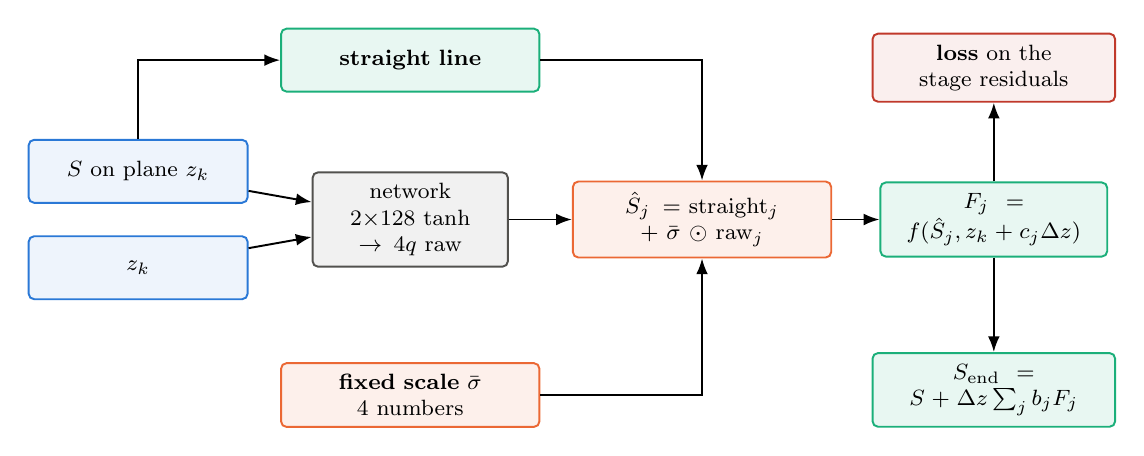
\begin{tikzpicture}[node distance=6mm and 6mm]
\node[inbox, text width=25mm] (S) {$S$ on plane $z_k$};
\node[inbox, text width=25mm, below=4mm of S] (z) {$z_k$};
\coordinate (m) at ($(S.east)!0.5!(z.east)$);
\node[netbox, text width=22mm, right=8mm of m] (body) {network\\2$\times$128 tanh\\$\to 4q$ raw};
\node[physbox, text width=30mm, above=10mm of body] (sl) {\textbf{straight line}};
\node[formbox, text width=30mm, below=12mm of body] (sc) {\textbf{fixed scale} $\bar\sigma$\\4 numbers};
\node[formbox, text width=30mm, right=8mm of body] (form) {$\Shat_j = $ straight$_j$\\$+\ \bar\sigma\odot\text{raw}_j$};
\node[physbox, text width=26mm, right=of form] (rates) {$F_j = f(\Shat_j, z_k + c_j\dz)$};
\node[physbox, text width=28mm, below=12mm of rates] (sum) {$S_{\text{end}} = S + \dz\sum_j b_jF_j$};
\node[lossbox, text width=28mm, above=10mm of rates] (loss) {\textbf{loss} on the stage residuals};
\draw[arr] (S) -- (body); \draw[arr] (z) -- (body);
\draw[arr] (S.north) |- (sl.west);
\draw[arr] (body) -- (form);
\draw[arr] (sl) -| (form.north);
\draw[arr] (sc) -| (form.south);
\draw[arr] (form) -- (rates);
\draw[arr] (rates) -- (sum);
\draw[arr] (rates) -- (loss);
\end{tikzpicture}
\end{center}

\begin{center}
\footnotesize
\begin{tabularx}{\textwidth}{@{}l X@{}}
\toprule
Prediction & The correction to the straight line, in units of $\bar\sigma$. At 64 steps $\bar\sigma = (0.0957\,\text{mm},\ 0.00085\,\text{mm},\ 0.00237,\ 0.0000209)$. \\
Configurations & 64 steps / 2 stages. \\
Everything else & As type 2. \\
\bottomrule
\end{tabularx}
\end{center}

\newpage
\section{Losses}

\textbf{Stage residual.} For training state $n$, stage $j$, component $d \in \{x, y, t_x, t_y\}$:
\[
r_{njd} = \Shat_{njd} - \dz\sum_{m=1}^{q} A_{jm}\, f_d\bigl(\Shat_{nm},\ z_n + c_m\dz\bigr) - S_{nd}.
\]
It is zero for all $n, j, d$ only when the stages solve the Gauss--Legendre equations. It has no label.

\subsection*{Pooled}
\[
\mathcal{L} = \operatorname*{mean}_{n,j,d}\ \Bigl(\frac{r_{njd}}{s_d}\Bigr)^2,
\]
$s_d$ = spread of component $d$ over the round-1 states.

\subsection*{Cost-weighted}
\[
\mathcal{L} = \operatorname*{mean}_{n,j,d}\ \Bigl(\frac{a_n\, g_{njd}\, r_{njd}}{D_{\text{ref}}}\Bigr)^2,
\qquad g_{nj} = (1,\ 1,\ \ell_{nj},\ \ell_{nj}),
\]
\begin{itemize}
\item $\ell_{nj} = z_1 - (z_n + c_j\dz) + \dz$: the distance left to travel, plus one step. A slope error is multiplied by it.
\item $D_n = \kappa\,|q/p|_n\, L \int |B|\,dz$: the total bend of track $n$ over the region.
\item $D_{\text{ref}}$: the median of $D_n$ over the round-1 states.
\item $a_n = \operatorname{clamp}\bigl(\sqrt{W(p_n)}\,D_{\text{ref}}/D_n,\ [m/5,\ 5m]\bigr)$, $m$ = batch median.
\item $W(p) = 1$ inside the momentum window, Gaussian in $\log p$ outside (width $\ln 2$), floor 0.05. Windows: 10--50\,GeV or 3--8\,GeV.
\end{itemize}

\section{Scores}

On the test tracks, against the reference. Radial error $\sqrt{\Delta x^2 + \Delta y^2}$.
\begin{itemize}
\item \textbf{End of region}: chain the network $N$ times from $z_0$; compare at $z_1$.
\item \textbf{Single step}: one step from the reference state on each start plane; compare with the reference one step later.
\end{itemize}

\end{document}
